% vim:nojs:spelllang=en_au tw=76 sw=4 sts=4 fo+=awn fmr={-{,}-} et ts=8
\documentclass[a4paper]{article}

\usepackage[T1]{fontenc}
\usepackage[utf8]{inputenc}
\usepackage{textcomp}
\usepackage{cite}
\usepackage[altbullet]{lucidabr}
\usepackage{siunitx}

\usepackage{tikz}
\usetikzlibrary{positioning,chains,matrix,shapes.arrows,scopes,
                shapes.misc,arrows,automata,calc,decorations.markings}

\usepackage[final,formats]{listings}
%\lstset{language=<...>,basicstyle=\sffamily}
\newcommand{\blue}[1]{\textbf{#1}}
\input{../../../tools/lst-zelus}

% see: http://www.tug.org/applications/hyperref/ftp/doc/manual.html
\usepackage[
    colorlinks=true,
    urlcolor=black,
    linkcolor=black,
    citecolor=black,
    pdfborder={0 0 0},
    pdfauthor={Timothy Bourke},
    pdftitle={},
    pdfsubject={},
    pdfkeywords={},
]{hyperref}

\pagestyle{empty}

\title{\vskip-2ex A slow afternoon chez PARKAS and a very fast fly (a fun 
talk)}
\author{Timothy Bourke$^{1,2}$
\and Marc Pouzet$^{2,1}$\\[1em]
\and 1. INRIA Paris-Rocquencourt
\and 2. École normale supérieure (DI)}
\date{Synchron Workshop, Dagstuhl, 19 November 2013}

\begin{document}
\maketitle

We briefly present a problem posed to use by Rafel Cases and Jordi 
Cortadella during a lunch organised by Gérard Berry.
We propose solutions in the Simulink 
tool\footnote{\url{http://www.mathworks.com/products/simulink/}} and our 
language Zélus\footnote{\url{http://zelus.di.ens.fr}}.

Imagine two cars.
One starts at Barcelona and travels at \SI{50}{\kilo\meter\per\hour} toward 
Girona---a distance of \SI{100}{\kilo\meter}.
The other starts at Girona and travels at \SI{50}{\kilo\meter\per\hour} 
toward Barcelona.
Between the two is a fly travelling at \SI{80}{\kilo\meter\per\hour}, 
initially from Barcelona toward Girona, and changing direction 
instantaneously whenever it meets either car.
There are two questions.
\begin{enumerate}

\item
How many zig-zags does the fly do during the two hours of travel?

\item
Where will the fly be when the two cars reach their destinations?

\end{enumerate}

We first modelled this problem in Simulink.
\begin{center}
\vskip-1em
\begin{tikzpicture}

  \clip (-6.1,-3.4) [rounded corners]rectangle (6.1,3.3);

  \node at (0,0) {
    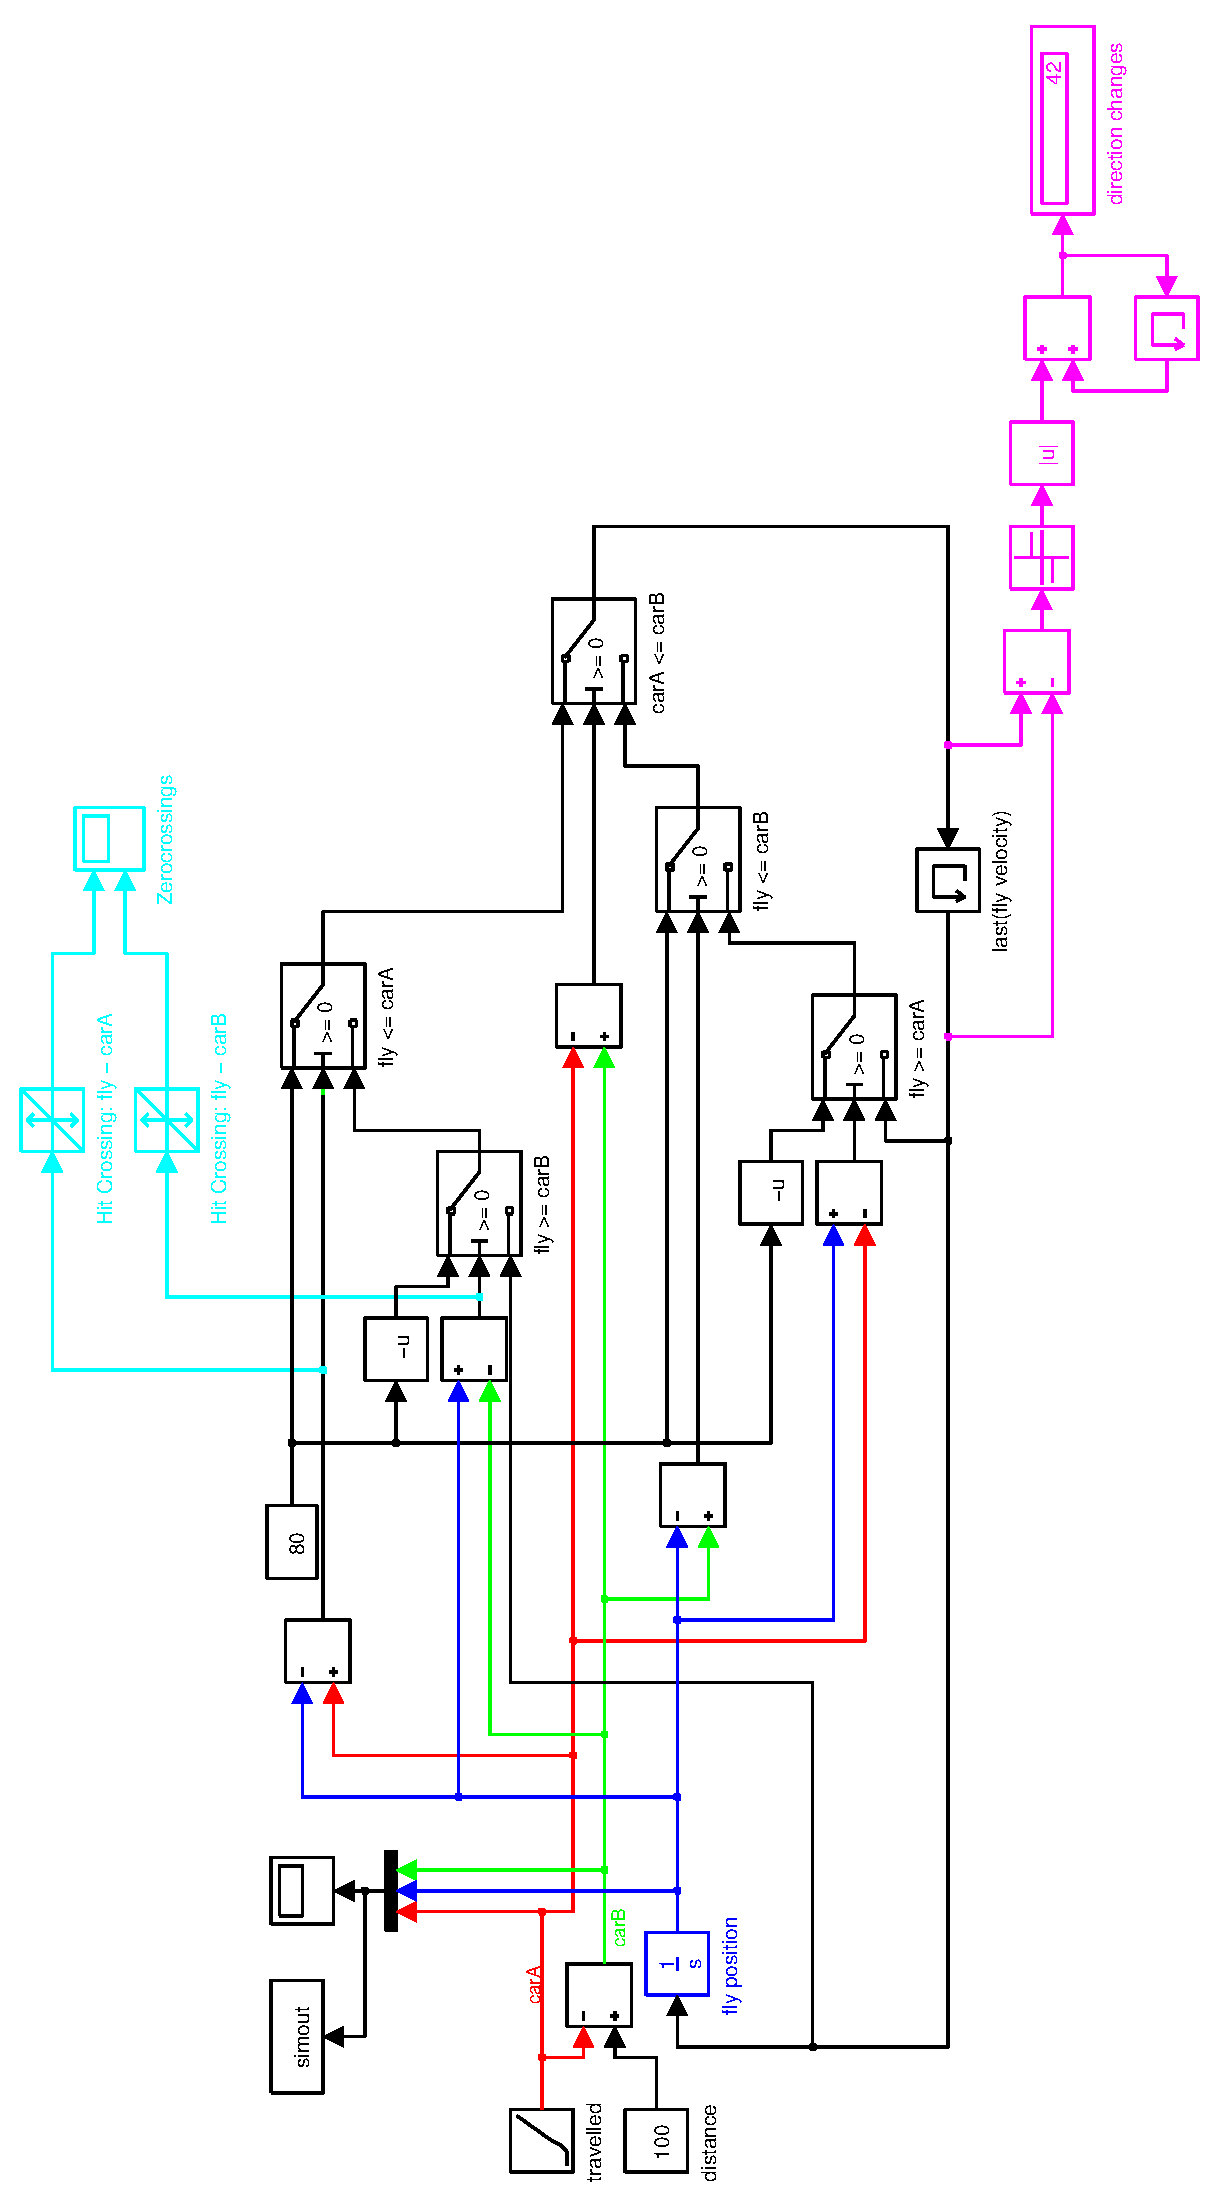
\includegraphics[width=6.8cm,angle=-90]{cantharide-sys.pdf}};

  \draw[red,very thick,->] (5.75,-1.8)
    node[left,red] {zigzags} -- +(0,-.5);

  \node[above right] (redcar) at (-5.8,.35)
    {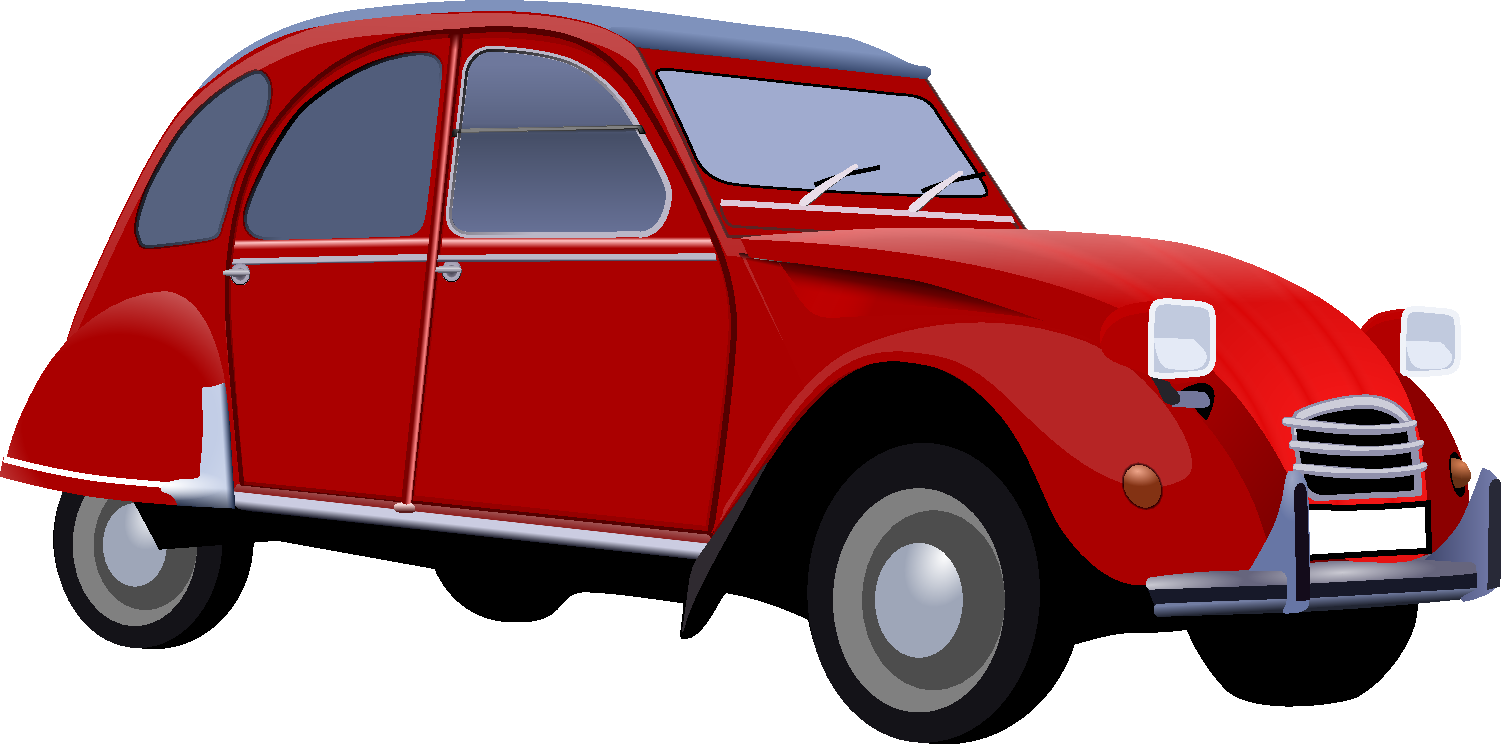
\includegraphics[width=.7cm,angle=0]{redcar.pdf}};
  \node[above right] (greencar) at (-4.7,-.5)
    {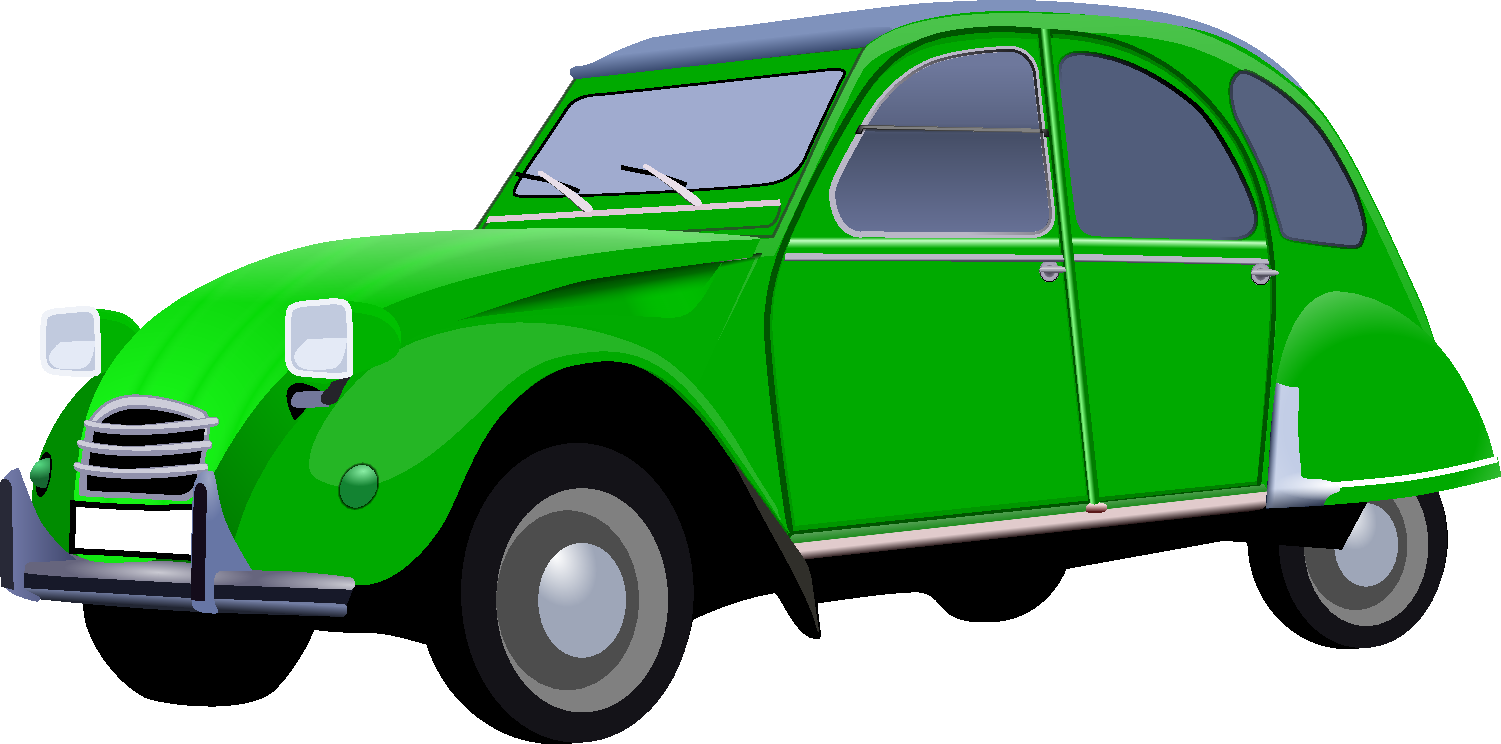
\includegraphics[width=.7cm,angle=0]{greencar.pdf}};
  \node[above right] (fly) at (-5.3,-1.6)
    {
\includegraphics[width=.7cm,angle=0]{fly.pdf}};

\end{tikzpicture}
\end{center}
The number of zig-zags, to our great surprise and pleasure, was 
\textbf{42}!~\cite{Adams:HG2G:1979} (Using R2012a with the ODE45 solver and 
a relative tolerance of $1\times10^{-3}$.)
\clearpage

We then modelled the problem in Zélus.
\begin{lst-zelus}{\footnotesize}
let barcelona = 0.0
let girona = 100.0

let fly_velocity = 80.0
let car_velocity = 50.0

let hybrid model () =  (car1, car2, fly, zigzag, zeros) where
  rec der car1 = car_velocity      init barcelona
  and der car2 = -. car_velocity init girona
  and der fly = dir *. fly_velocity init barcelona
  and automaton
        | Above ->
             do car_above = car2
             and car_below = car1
             until up(car1 -. car2) then Below
        | Below -> 
             do car_above = car1
             and car_below = car2
             done
        end
  and present 
         up (car_below -. fly) | up(fly -. car_above) -> 
           do
              dir = -. (last dir)
              and zeros = last zeros + 1
              and emit zigzag = ()
           done
  and init dir = 1.0
  and init zeros = 0
\end{lst-zelus}
This gave an answer of \textbf{48} and the graph shown below.
(Using the Sundials CVODE solver and a custom implementation of the Illinois 
algorithm.)

\begin{center}
\scalebox{.81}{
\begin{tikzpicture}

\clip (-6.1,-3.4) [rounded corners]rectangle (6.1,3.6);

\node at (0,0) {
  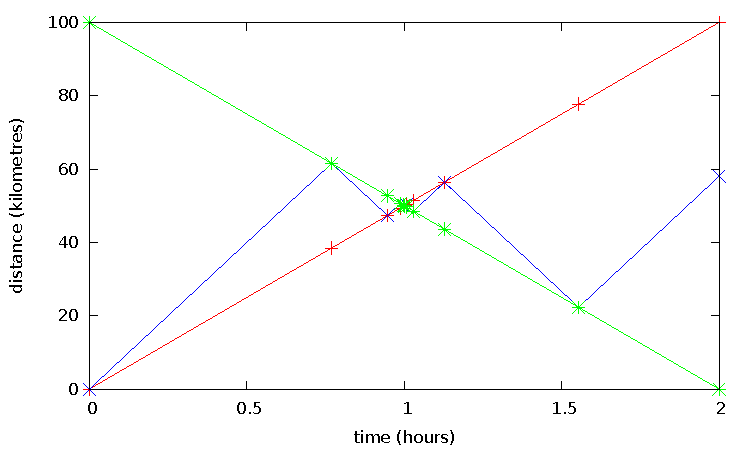
\includegraphics[width=.95\textwidth]{zelus.pdf}};

\node[above right] (redcar) at (-5.70,-3.1)
  {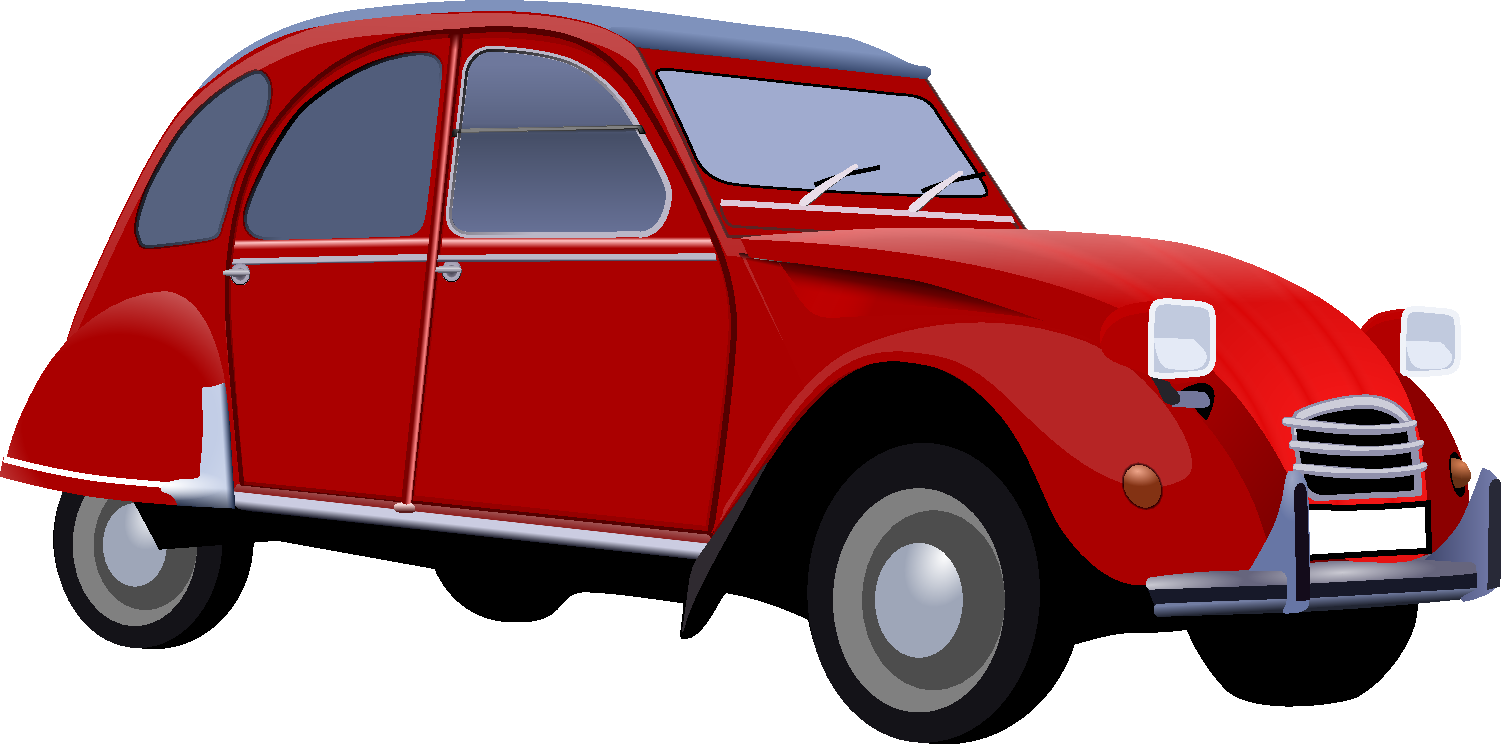
\includegraphics[width=.7cm,angle=90]{redcar.pdf}};
\node[above right] (greencar) at (-5.75,2.5)
  {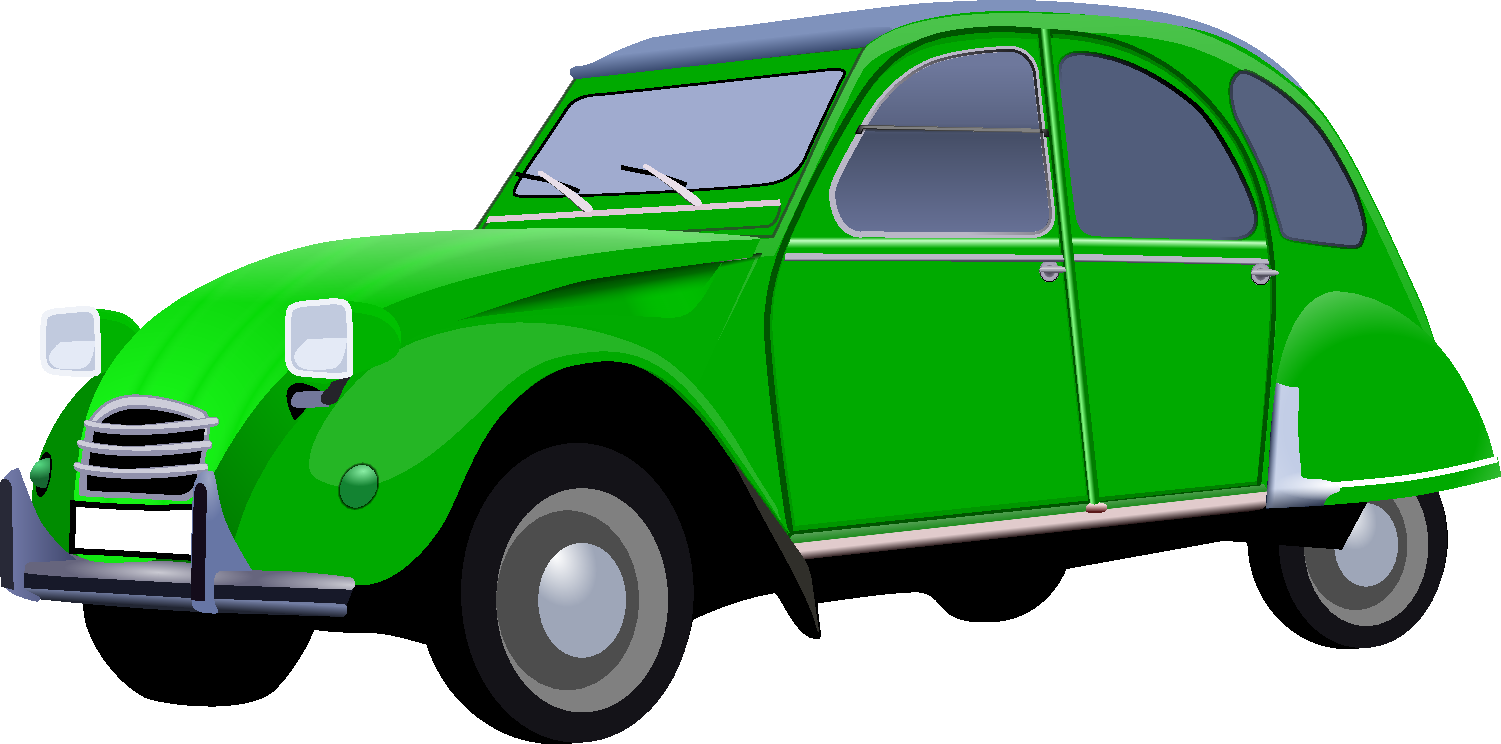
\includegraphics[width=.7cm,angle=90]{greencar.pdf}};
\node[below left] at (-5.0,-3.0) {\tiny{Barcelona}};
\node[below left] at (-5.0,3.7) {\tiny{Girona}};
\node[above right] (fly) at (-4.4,-2.2)
  {
\includegraphics[width=.7cm,angle=0]{fly.pdf}};

\end{tikzpicture}}
\end{center}

Obviously neither answer is correct since the system is not well defined at 
the instant the cars pass each other.
The important questions are whether we should, or even can, statically 
detect and reject such cases? or stop with an error at runtime?

\bibliographystyle{abbrv}
\bibliography{synchron2013}
\end{document}
